\documentclass[11pt]{article}

\usepackage[margin=1in]{geometry}
\usepackage{amsmath,amssymb,amsthm}
\usepackage{booktabs}
\usepackage{graphicx}
\graphicspath{{../figures/}}
\usepackage{xcolor}
\usepackage{subcaption}
\usepackage{algorithm}
\usepackage{algpseudocode}
\usepackage{multirow}
\usepackage{hyperref}
\usepackage{cite}

\newtheorem{theorem}{Theorem}
\newtheorem{proposition}[theorem]{Proposition}
\newtheorem{corollary}[theorem]{Corollary}
\newtheorem{remark}[theorem]{Remark}
\newtheorem{assumption}{Assumption}

% Custom commands
\newcommand{\Cs}{C_s}
\newcommand{\fmax}{f_{\max}}
\newcommand{\sstar}{s^{*}}
\newcommand{\pfault}{p_{\text{fault}}}
\newcommand{\rhoeff}{\rho_{\text{eff}}}
\newcommand{\tbase}{t_{\text{base}}}
\newcommand{\system}{\textsc{Prism}}

\begin{document}

\title{Capacity-Theoretic Limits of Slow Fault Mitigation\\under Power-of-Two-Choices Routing}
\author{DaLaw2}
\date{}
\maketitle

\begin{abstract}
Slow faults---where nodes remain reachable but exhibit degraded
performance---are a persistent source of tail latency violations in
distributed systems. Unlike crash faults, slow faults evade health checks
and produce ambiguous signals under high load. We present a
capacity-theoretic analysis of slow fault mitigation under
Power-of-Two-Choices (P2C) load balancing, establishing three results.
First, the \emph{operating envelope}: the maximum tolerable fault fraction
is $\fmax = 1 - L/U$, where $L$ is the load factor and $U$ the
utilization ceiling, validated empirically with zero fitted parameters.
Second, \emph{severity non-monotonicity}: under P2C routing, a moderate
slowdown (e.g., 10$\times$) causes worse tail latency than an extreme one
(e.g., 20$\times$), with the critical severity $\sstar =
fq/((1-q)(N-f))$. Third, \emph{SHED--P2C complementarity}: P2C's
queue-depth comparison and explicit weight reduction (SHED) are
complementary mechanisms operating at different stages of routing---SHED
provides 5--70\,ms P99 improvement at moderate severity ($2$--$5\times$)
but is unnecessary above $\sstar$ where P2C self-isolates faulty nodes.
Crucially, any detection-triggered weight reduction achieves nearly
identical results to full isolation under P2C, demonstrating that
\emph{detection speed, not response strategy, is the primary bottleneck}
in slow fault mitigation. Through discrete-event simulation across 15
fault scenarios, we show that reactive mechanisms (hedged requests, timeout
retry) are ineffective, while proactive detection with traffic exclusion is
necessary and sufficient. Our results provide practitioners with analytical
tools to determine when mitigation is feasible, which severity regime
demands intervention, and why detection precision matters less than
detection speed under queue-aware routing.
\end{abstract}

\section{Introduction}
\label{sec:intro}

Slow faults---where a node remains reachable but exhibits degraded
performance---are among the most insidious failures in distributed
systems~\cite{huang2017gray, gunawi2018fail}. Unlike crash faults, which
are detected immediately by health checks, slow faults produce ambiguous
signals: elevated latency that may stem from transient load rather than
genuine degradation. Left unmitigated, a single slow node in a cluster of
32 can increase system P99 latency by 3--9$\times$, violating
service-level objectives (SLOs) and propagating through dependency
chains~\cite{dean2013tail}.

The standard response to tail latency is \emph{hedged requests}: send a
speculative copy to a second server after a brief delay, and use whichever
response arrives first~\cite{dean2013tail}. This works well for
\emph{random stragglers}---transient delays caused by garbage collection,
context switching, or background I/O. However, persistent slow faults
differ fundamentally: the same nodes remain slow across thousands of
requests, rendering per-request hedging ineffective because future requests
continue to be routed to faulty nodes.

Modern load balancers predominantly use Power-of-Two-Choices (P2C)
routing~\cite{mitzenmacher2001power}, which samples two candidates weighted
by their routing weights and selects the one with the shorter queue. A
natural question arises: \emph{does P2C's queue-depth awareness already
handle slow faults, making explicit mitigation redundant?} In this paper,
we answer this question with three theoretical results and extensive
empirical validation.

\begin{enumerate}
\item \textbf{Operating envelope.} The maximum fraction of faulty nodes
  that any mitigation strategy can tolerate is:
  \begin{equation}
    \fmax = 1 - \frac{L}{U}
    \label{eq:envelope}
  \end{equation}
  where $L$ is the system load factor and $U \approx 0.89$ is the
  utilization ceiling beyond which M/D/1 queueing delay grows
  superlinearly. This formula, with \emph{zero fitted parameters}, predicts
  the empirical pass/fail boundary across four load levels
  (Section~\ref{sec:envelope}).

\item \textbf{Severity non-monotonicity.} Under P2C routing, the ``worst''
  slowdown factor is not the highest but the one where the fraction of
  traffic reaching faulty nodes exactly equals the percentile tail width:
  \begin{equation}
    \sstar = \frac{f \cdot q}{(1-q)(N-f)}
    \label{eq:sstar}
  \end{equation}
  Above $\sstar$, P2C's queue-depth comparison renders faulty requests
  statistically invisible---the system \emph{self-isolates} the faulty
  node without any explicit intervention
  (Section~\ref{sec:nonmono}).

\item \textbf{SHED--P2C complementarity.} P2C routing and explicit weight
  reduction (SHED) operate at different stages of the routing decision:
  SHED controls \emph{candidate selection probability} while P2C provides
  a \emph{queue-depth tiebreaker}. These are complementary, not redundant.
  SHED's benefit scales as $O(N^{-\alpha})$ ($\alpha \approx 1.3$),
  is maximized at moderate severity ($2$--$5\times$), and vanishes above
  $\sstar$ where P2C self-isolates. Crucially, under P2C a minimum weight
  of $w_{\min} = 0.05$ achieves nearly identical P99 to full isolation
  ($w = 0$), demonstrating that \emph{detection accuracy matters far less
  than detection speed} (Section~\ref{sec:complementarity}).
\end{enumerate}

We validate these results through discrete-event simulation of clusters
ranging from 8 to 64 nodes across 15 fault scenarios. Our evaluation
compares eight mitigation strategies, including three literature baselines
(hedged requests~\cite{dean2013tail}, outlier
blacklisting~\cite{lakshman2010cassandra}, and timeout retry). The key
empirical findings are:

\begin{itemize}
\item \textbf{Detection speed is the primary bottleneck.} Under P2C routing,
  graduated weight reduction and full isolation produce nearly identical
  P99 latency (gap $< 2$\,ms). The response strategy is inconsequential
  once detection identifies the faulty node. This holds across cluster
  sizes, severity levels, and load factors (Section~\ref{sec:eval-shed}).

\item \textbf{Reactive mechanisms fail.} Hedged requests and timeout retry
  improve SLO compliance by less than 0.3 percentage points over no
  mitigation---they are designed for random stragglers, not persistent
  faults (Section~\ref{sec:eval-lit}).

\item \textbf{Proactive detection is necessary and sufficient.} All
  strategies that detect faulty nodes and redirect traffic achieve P99
  $< 45$\,ms across all scenarios at 80\% load, regardless of the specific
  response strategy (SHED vs.\ isolation). The gap between no mitigation
  and any proactive strategy (5--70\,ms) dwarfs the gap between different
  proactive strategies ($< 2$\,ms) (Section~\ref{sec:eval-tiers}).
\end{itemize}

Our contributions provide practitioners with: (1)~a simple formula to
determine whether mitigation is feasible for a given load and fault
fraction; (2)~an analytical tool to identify the most dangerous slowdown
regime; (3)~a complementarity theorem explaining when P2C suffices alone
and when explicit detection is needed; and (4)~empirical evidence that
detection speed, not response precision, is the primary design target for
slow fault mitigation systems.

\section{Background and Motivation}
\label{sec:background}

\subsection{Slow Faults in Production Systems}

Gray failures~\cite{huang2017gray} encompass a spectrum of partial
failures where components are neither fully operational nor completely
down. Slow faults---a subclass where service time degrades by a factor
$s > 1$---arise from diverse root causes: memory pressure causing
excessive garbage collection, disk degradation increasing I/O latency,
thermal throttling reducing CPU frequency, or network congestion on a
specific path~\cite{gunawi2018fail}.

Unlike crash faults, slow faults are difficult to detect because the
affected node continues to respond, albeit slowly. Standard health
checks (TCP probes, heartbeats) cannot distinguish a 5$\times$ slower
node from a healthy one under transient load. This ambiguity is
especially pronounced at high system utilization, where \emph{all} nodes
exhibit elevated latency due to queueing effects.

\subsection{Power-of-Two-Choices Load Balancing}

Power-of-Two-Choices (P2C)~\cite{mitzenmacher2001power} is the dominant
load balancing algorithm in modern distributed systems, used in
Envoy~\cite{envoy}, nginx, and numerous cloud-native
infrastructure. For each incoming request, P2C samples two candidate
workers at random and routes the request to the one with the shorter
queue.

P2C provides an important but under-appreciated implicit mitigation
mechanism for slow faults. A node with slowdown factor $s$ processes
requests $s$ times slower, causing its queue to grow. P2C's queue-depth
comparison then naturally avoids this node, routing traffic to healthier
alternatives. We show in Section~\ref{sec:nonmono} that this implicit
mitigation is highly effective at extreme severities ($s > \sstar$) but
insufficient at moderate severities ($s < \sstar$), precisely where
explicit mitigation strategies add value.

\subsection{Existing Mitigation Approaches}

\paragraph{Hedged requests.}
Dean and Barroso~\cite{dean2013tail} proposed sending a speculative
copy of a request to a second server after a delay (typically the
expected service time). The client uses whichever response arrives
first. This is effective for random stragglers but, as we demonstrate,
ineffective for persistent slow faults because new requests continue to
be routed to the faulty node.

\paragraph{Outlier blacklisting.}
Systems like Cassandra's dynamic snitch~\cite{lakshman2010cassandra}
track per-node latency and temporarily blacklist nodes whose latency
exceeds $k$ standard deviations above the cluster median. This is a
proactive mechanism that redirects future traffic, but risks oscillation
at high load when blacklisting reduces capacity and increases latency on
remaining nodes.

\paragraph{Circuit breaking.}
Istio and Envoy implement circuit breakers that open when error rates or
latency exceed thresholds, redirecting traffic away from unhealthy
endpoints. These are effective but require manual threshold tuning and
do not adapt to varying load conditions.

\subsection{The Mitigation Trap}
\label{sec:trap}

A key motivation for this work is the \emph{mitigation trap}: at high
system load, naive mitigation strategies can be \emph{worse than doing
nothing}. Consider hedged requests at 85\% load: each hedge adds a
duplicate request, pushing healthy workers from $\rho = 0.85$ toward
saturation. The M/D/1 queueing delay grows as $\rho/(2(1-\rho))$,
creating a positive feedback loop: hedges increase load, which
increases latency, which triggers more hedges.

We discovered this phenomenon empirically (Section~\ref{sec:eval-lit})
and it motivates the load-aware design of our adaptive framework: any
mitigation strategy must account for its own capacity cost.

\section{System Model}
\label{sec:model}

\subsection{Architecture}

We model a single-tier distributed service consisting of $N$
homogeneous worker nodes fronted by a load balancer. Requests arrive as
a Poisson process with aggregate rate $\Lambda = L \cdot N \cdot \mu$,
where $L \in (0, 1)$ is the \emph{load factor} and $\mu = 1/\tbase$ is
the per-node service rate. Each worker processes requests sequentially
(single-server) with deterministic service time $\tbase$ under normal
conditions, yielding an M/D/1 queueing model per node.

The load balancer implements weighted Power-of-Two-Choices (P2C): for
each request, it samples two candidates with probability proportional
to their weights $w_i \in [0, 1]$ and routes to the candidate with the
shorter queue depth.

\subsection{Fault Model}

A \emph{slow fault} on node $i$ multiplies its service time by a
slowdown factor $s_i > 1$:
\begin{equation}
  t_i = s_i \cdot \tbase
\end{equation}
We consider $f$ simultaneously faulty nodes out of $N$ total. Faults
are \emph{persistent}: once onset occurs, the slowdown remains until
explicit recovery (if any). We study five fault patterns:

\begin{itemize}
\item \textbf{Permanent}: constant $s$ after onset.
\item \textbf{Progressive}: $s(t) = 1 + (s_{\max}-1)(1-e^{-\beta t})$,
  gradually worsening.
\item \textbf{Fluctuating}: alternates between $s = s_{\text{peak}}$ and
  $s = 1$ with configurable on/off durations.
\item \textbf{Cascading}: faults appear sequentially on different nodes
  at staggered times.
\item \textbf{Recovering}: fault active for a fixed duration, then node
  returns to normal.
\end{itemize}

\subsection{Performance Metrics}

We evaluate using standard tail latency metrics:
\begin{itemize}
\item \textbf{P99/P999 latency}: 99th and 99.9th percentile of
  end-to-end request latency (including queueing delay).
\item \textbf{SLO violation rate}: fraction of requests exceeding the
  SLO target (50\,ms in our experiments).
\item \textbf{Goodput}: requests completing within SLO per second.
\item \textbf{Affected ratio}: fraction of requests served by faulty
  nodes (measures load balancer effectiveness).
\end{itemize}

\subsection{Minimax Regret}

To compare strategies across diverse scenarios, we use the \emph{minimax
regret} criterion. For strategy $j$ in scenario $i$, the regret is:
\begin{equation}
  R_{ij} = P99_{ij} - \min_k P99_{ik}
\end{equation}
The minimax regret of strategy $j$ is $\max_i R_{ij}$: its worst-case
gap from the best strategy in any scenario. A strategy with low minimax
regret is robust across operating conditions.

\section{Analytical Results}
\label{sec:analysis}

We derive three results that characterize the fundamental limits and
mechanisms of slow fault mitigation under P2C routing.

\subsection{Operating Envelope}
\label{sec:envelope}

When the detector isolates faulty nodes, the load on the remaining
healthy nodes rises. Intuitively, there is a tipping point---isolate
too many nodes, and the healthy nodes themselves become overloaded.
The following theorem quantifies this tipping point.

\begin{theorem}[Operating Envelope]
\label{thm:envelope}
In a cluster of $N$ nodes at load factor $L$, the maximum fraction of
faulty nodes that can be tolerated by any isolation-based mitigation
strategy is:
\begin{equation}
  \fmax = 1 - \frac{L}{U}
\end{equation}
where $U$ is the utilization ceiling beyond which per-node queueing
delay becomes unacceptable.
\end{theorem}

\begin{proof}
When $f$ nodes are isolated (removed from the active pool), the
remaining $N - f$ healthy nodes must absorb the entire system load. The
effective per-node utilization becomes:
\begin{equation}
  \rhoeff = \frac{\Lambda}{(N-f) \cdot \mu} = \frac{L \cdot N}{N - f}
\end{equation}
For the system to remain stable with acceptable queueing delay, we
require $\rhoeff \leq U$. Solving for $f$:
\begin{equation}
  f \leq N \left(1 - \frac{L}{U}\right)
\end{equation}
\end{proof}

In short, $L/U$ is the minimum fraction of nodes needed to sustain the
load; anything beyond that is the margin available for isolation.
The higher the load, the smaller the margin.

\medskip

The parameter $U$ in Theorem~\ref{thm:envelope} is free---it depends
on how ``acceptable queueing delay'' is defined. We next derive its
closed form from the M/D/1 model, turning the envelope into a
zero-parameter prediction tool.
For a single-server queue with deterministic service time $\tbase$,
the mean sojourn time is:
\begin{equation}
  T(\rho) = \tbase \cdot \frac{2 - \rho}{2(1 - \rho)}
  \label{eq:md1}
\end{equation}
Rather than choosing $U$ empirically, we derive it from the SLO
constraint $T(U) \leq \text{SLO}$.

\begin{corollary}[Closed-Form Utilization Ceiling]
\label{cor:U}
For an M/D/1 queue with base service time $\tbase$ and a mean-latency
SLO target, the utilization ceiling is:
\begin{equation}
  U = 1 - \frac{\tbase}{2 \cdot \text{SLO} - \tbase}
    = \frac{2(\text{SLO} - \tbase)}{2 \cdot \text{SLO} - \tbase}
  \label{eq:U}
\end{equation}
\end{corollary}

\begin{proof}
Set $T(U) = \text{SLO}$ in Equation~\ref{eq:md1},
let $\alpha = 2\,\text{SLO}/\tbase$, and solve the resulting linear
equation to obtain
$U = (\alpha - 2)/(\alpha - 1) = 1 - \tbase/(2 \cdot \text{SLO} - \tbase)$.
\end{proof}

For our parameters ($\text{SLO} = 50$\,ms, $\tbase = 10$\,ms):
$U = 1 - 10/90 = 8/9 \approx 0.889$. We use $U = 8/9$ throughout.

\medskip

\paragraph{Generalization to M/G/1 service times.}
The following generalization is not required for the main argument,
but quantifies the impact of service-time variability on the envelope.
When service times are variable with coefficient of variation $\Cs$,
the Pollaczek--Khinchine formula gives:
\begin{equation}
  T(\rho) = \tbase \left[1 + \frac{(1 + \Cs^2)\,\rho}{2(1-\rho)}\right]
  \label{eq:mg1}
\end{equation}
Solving $T(U) = \text{SLO}$ yields the generalized ceiling:
\begin{equation}
  U(\Cs) = \frac{\alpha}{\alpha + 1 + \Cs^2}
  \quad\text{where } \alpha = 2\left(\frac{\text{SLO}}{\tbase} - 1\right)
  \label{eq:U_mg1}
\end{equation}

Table~\ref{tab:Ucv} shows the impact of service-time variability.

\begin{table}[t]
\centering
\caption{Mean-latency-based utilization ceiling $U$ and operating
  envelope $\fmax$ at $L = 0.80$ for different service-time
  distributions. Values are derived from the constraint
  $T_{\text{mean}}(U) \leq \text{SLO}$.}
\label{tab:Ucv}
\begin{tabular}{@{}llccc@{}}
\toprule
Distribution & $\Cs^2$ & $U$ & $\fmax$ & Max faults ($N{=}32$) \\
\midrule
M/D/1 & 0 & 0.889 & 10.0\% & 3.2 \\
M/G/1 (mild) & 0.25 & 0.865 & 7.5\% & 2.4 \\
M/M/1 & 1.0 & 0.800 & 0.0\% & 0.0 \\
\bottomrule
\end{tabular}
\end{table}

The M/M/1 case ($\Cs^2 = 1$) is striking: $U = 0.800$, meaning at
$L = 0.80$ there is \emph{zero} fault tolerance. Any slow fault
immediately violates the SLO. This quantifies the well-known
intuition that service-time variability erodes system headroom, and
shows that the deterministic M/D/1 assumption provides an optimistic
bound on fault tolerance.

\begin{remark}[Validity and Tightness of the Mean-Based Ceiling]
\label{rem:mean-p99}
\label{rem:tight}
Table~\ref{tab:Ucv} derives $U$ from mean latency, but SLOs are
typically defined at P99.
For M/D/1 ($\Cs^2 = 0$), the gap is small: deterministic service
times produce low response-time variance, so
$U_{\text{P99}} \gtrsim U_{\text{mean}}$ and the formula is
\emph{conservative} (safe).
For M/M/1 ($\Cs^2 = 1$), the gap is large: simulation shows P99
crosses a 50\,ms SLO at $L \approx 0.70$, so the mean-based $U$ is
\emph{optimistic} for high-variance distributions.
In terms of tightness, at $L = 0.80$, $N = 32$ the theoretical limit
is 3.2 nodes, yet experiments pass with 4 isolated nodes achieving
P99 $< 50$\,ms. This margin arises from the gap between mean latency
and P99. The envelope is slightly conservative, with the pass/fail
boundary error within one to two nodes.
\end{remark}

\paragraph{Non-isolation strategies.}
The bound in Theorem~\ref{thm:envelope} assumes faulty nodes are fully
isolated. Strategies that \emph{reduce} traffic to faulty nodes (load
shedding) without fully isolating them achieve a tighter effective
capacity: the faulty node contributes $\mu/s_i$ effective service rate.
In this case:
\begin{equation}
  \rhoeff = \frac{L \cdot N}{(N-f) + \sum_{i \in F} 1/s_i}
\end{equation}
where $F$ is the set of faulty nodes. This is always lower than the
isolation case, confirming that the operating envelope bound is
\emph{conservative}: non-isolation strategies can tolerate slightly
higher fault fractions by preserving partial capacity.

\paragraph{Empirical validation.}
We validate Equation~\ref{eq:envelope} across four load levels with
$N = 32$ and permanent 5$\times$ faults (Table~\ref{tab:envelope}).

\begin{table}[t]
\centering
\caption{Operating envelope validation. Theory predicts the maximum
  fault fraction; empirical column shows whether the adaptive strategy
  achieves P99 $< 50$\,ms SLO.}
\label{tab:envelope}
\begin{tabular}{@{}ccccl@{}}
\toprule
$L$ & $\fmax$ & $f_{\max}$ nodes & Empirical boundary & Match \\
\midrule
0.70 & 21.3\% & 6.8 & 8 pass, 10 fail & \checkmark$^\dagger$ \\
0.80 & 10.0\% & 3.2 & 4 pass, 6 fail & \checkmark \\
0.85 & 4.4\% & 1.4 & 2 pass, 4 fail & \checkmark$^\dagger$ \\
0.90 & $<0$ & --- & 0 pass, 2 fail & \checkmark \\
\bottomrule
\end{tabular}
\end{table}

The formula predicts the pass/fail boundary with zero fitted
parameters. Rows marked $\dagger$ show the empirical boundary
exceeding the theoretical maximum (e.g., 8 nodes pass at $L=0.70$
despite a theoretical limit of 6.8), because $U$ is derived from
\emph{mean} latency while P99's effective ceiling is slightly higher
(Remark~\ref{rem:mean-p99}), making the envelope a conservative
estimate. At $L = 0.90$, the load exceeds $U = 8/9$ and SLO
compliance fails even without faults.

Figure~\ref{fig:envelope} visualizes the operating envelope across load
levels, showing the sharp boundary between the SAFE and OVERLOAD zones.

\begin{figure}[t]
\centering
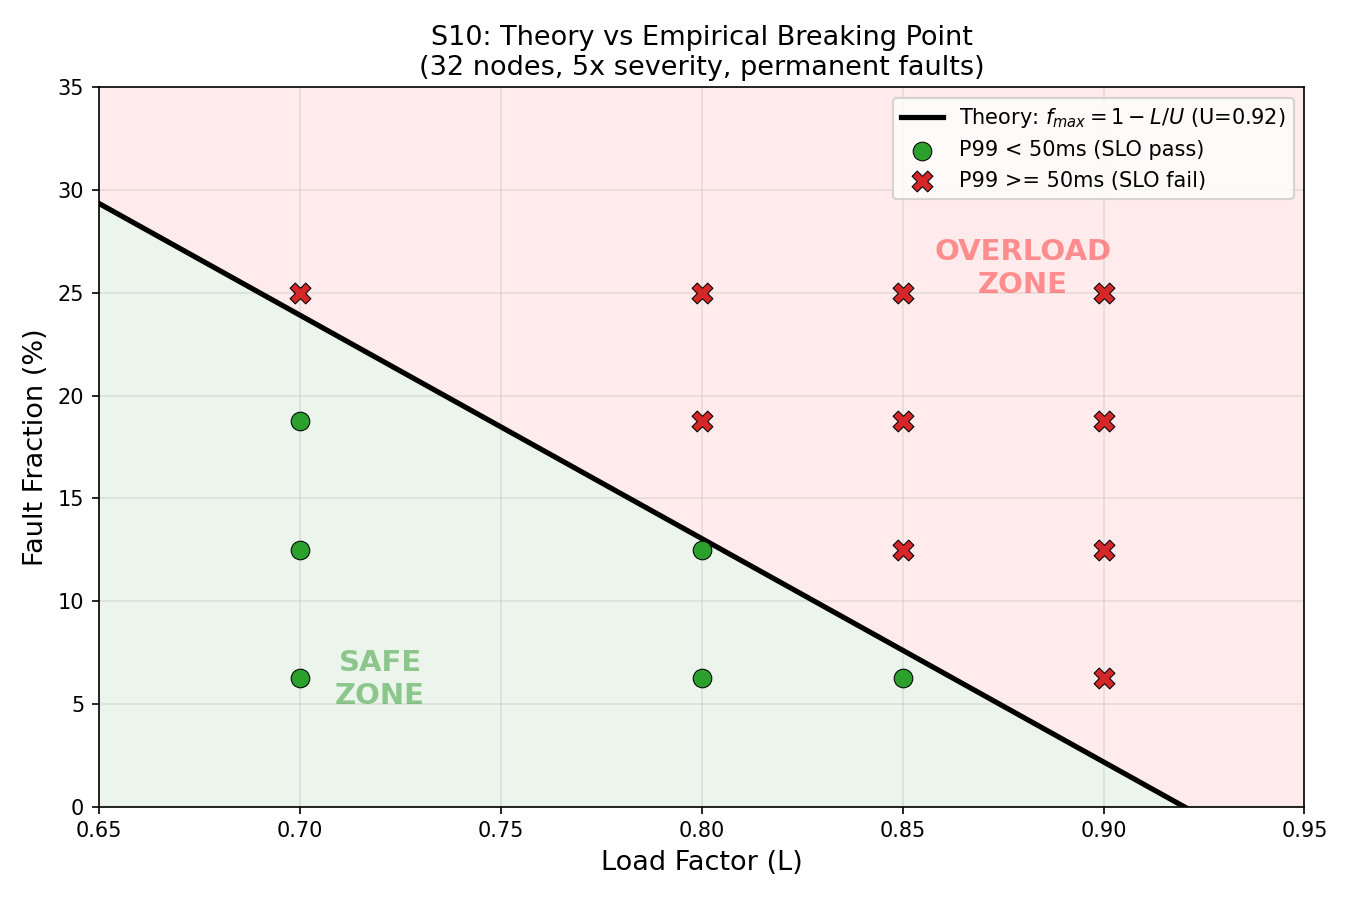
\includegraphics[width=0.85\linewidth]{operating_envelope.png}
\caption{Operating envelope: theory vs.\ empirical. The boundary
  $\fmax = 1 - L/U$ (dashed line) separates the SAFE zone (P99
  $< 50$\,ms) from the OVERLOAD zone, validated with zero fitted
  parameters.}
\label{fig:envelope}
\end{figure}

\subsection{Severity Non-Monotonicity}
\label{sec:nonmono}

\begin{assumption}[Mean-Field P2C Approximation]
\label{asm:meanfield}
Under P2C with weighted random sampling, traffic to each node is
proportional to its effective service capacity in steady state. That
is, a node with capacity $\mu_i$ receives a fraction
$\mu_i / \sum_j \mu_j$ of the total traffic.
\end{assumption}

This approximation is exact when the number of nodes is large and
sampling is capacity-weighted. For finite clusters, P2C's
queue-depth tie-breaking introduces a small positive bias toward
faulty nodes (see Table~\ref{tab:pfault}: underestimates by 10--14\%
at $f = 4$, $< 1$\% at $f = 8$).

\medskip

\begin{theorem}[Critical Severity]
\label{thm:sstar}
Under Assumption~\ref{asm:meanfield}, the
fraction of traffic reaching $f$ faulty nodes with slowdown $s$ is:
\begin{equation}
  \pfault(f, s, N) = \frac{f}{s \cdot (N-f) + f}
  \label{eq:pfault}
\end{equation}
The critical severity at which faulty traffic becomes invisible to the
$q$-th percentile is:
\begin{equation}
  \sstar = \frac{f \cdot q}{(1-q)(N-f)}
  \label{eq:sstar_deriv}
\end{equation}
\end{theorem}

In other words: P2C routing assigns less traffic to more severely
faulty nodes. When the severity is high enough, the faulty traffic
fraction drops below $1-q$---at which point faulty requests become
statistically invisible at the $q$-th percentile.
$\sstar$ is precisely this tipping point.

\begin{proof}
Under P2C, traffic is proportional to effective service capacity.
Healthy nodes have capacity $\mu$; faulty nodes have $\mu/s$.
The faulty traffic fraction simplifies to
$\pfault = f / [s(N{-}f) + f]$ (Equation~\ref{eq:pfault}).
The system latency follows a mixture distribution;
faulty requests are visible at percentile $q$ when $\pfault > 1-q$.
Setting $\pfault = 1-q$ and solving for $s$ yields $\sstar$.
\end{proof}

\medskip

\paragraph{Non-monotonicity mechanism.}
For $s < \sstar$: $\pfault > 1-q$, so faulty-node latency dominates the
$q$-th percentile. The system $P_q$ increases with $s$ because faulty
service time $= s \cdot \tbase$.

For $s > \sstar$: $\pfault < 1-q$, so faulty requests are statistically
invisible in the $q$-th percentile. The system $P_q$ drops back to the
healthy-node value.

The \emph{worst} $P_q$ therefore occurs near $s = \sstar$, not at
$s \to \infty$. This is the severity non-monotonicity: increasing the
fault severity beyond $\sstar$ paradoxically \emph{improves} the
observed tail latency.

This means that the most challenging scenario for operators is not
an extreme fault ($s \gg \sstar$) but a moderate one
($s \approx \sstar$)---precisely the regime that is hardest to detect.

\paragraph{Percentile-dependent risk.}
The same fault configuration can be simultaneously invisible to one
percentile and visible to another. For $f = 4$, $N = 32$:
$s^{*}_{P99} = 14.1$ but $s^{*}_{P999} = 142.7$. A 20$\times$
slowdown is invisible to P99 ($20 > 14.1$) but visible to P999
($20 < 142.7$), explaining the observed pattern: P99 $= 49$\,ms
(normal) but P999 $= 17{,}427$\,ms (catastrophic).

\paragraph{Empirical validation.}
Table~\ref{tab:pfault} validates the traffic distribution model.

\begin{table}[t]
\centering
\caption{Traffic fraction reaching faulty nodes: theory vs.\ empirical
  (no mitigation, $N=32$, $L=0.80$).}
\label{tab:pfault}
\begin{tabular}{@{}ccccc@{}}
\toprule
$f$ & $s$ & Theory $\pfault$ & Empirical & Ratio \\
\midrule
4 & 3$\times$ & 4.55\% & 5.20\% & 1.14 \\
4 & 5$\times$ & 2.78\% & 3.12\% & 1.12 \\
4 & 10$\times$ & 1.41\% & 1.56\% & 1.11 \\
4 & 20$\times$ & 0.71\% & 0.78\% & 1.10 \\
\midrule
8 & 3$\times$ & 10.00\% & 10.42\% & 1.04 \\
8 & 5$\times$ & 6.25\% & 6.26\% & 1.00 \\
8 & 10$\times$ & 3.23\% & 3.23\% & 1.00 \\
8 & 20$\times$ & 1.64\% & 1.64\% & 1.00 \\
\bottomrule
\end{tabular}
\end{table}

The model systematically underestimates by 10--14\% at $f=4$ (due to
P2C's queue-depth tie-breaking sending slightly more traffic to slower
nodes than the mean-field model predicts) and is exact to three
significant figures at $f=8$.
The systematic positive bias at $f = 4$ (ratio $\approx 1.10$--$1.14$)
arises from P2C's queue-depth tie-breaking; the residual bias scales
as $O(1/N)$.
For practical purposes, the mean-field approximation is sufficient to
predict the critical severity $\sstar$ and the P99 visibility boundary.

Figure~\ref{fig:heatmap} shows the severity non-monotonicity across
fault count and slowdown factor combinations. The heatmap clearly
shows that moderate severities (e.g., $10\times$ with 4 faults:
P99 $= 439$\,ms) produce worse tail latency than extreme severities
(e.g., $20\times$ with 4 faults: P99 $= 49$\,ms).

\begin{figure}[t]
\centering
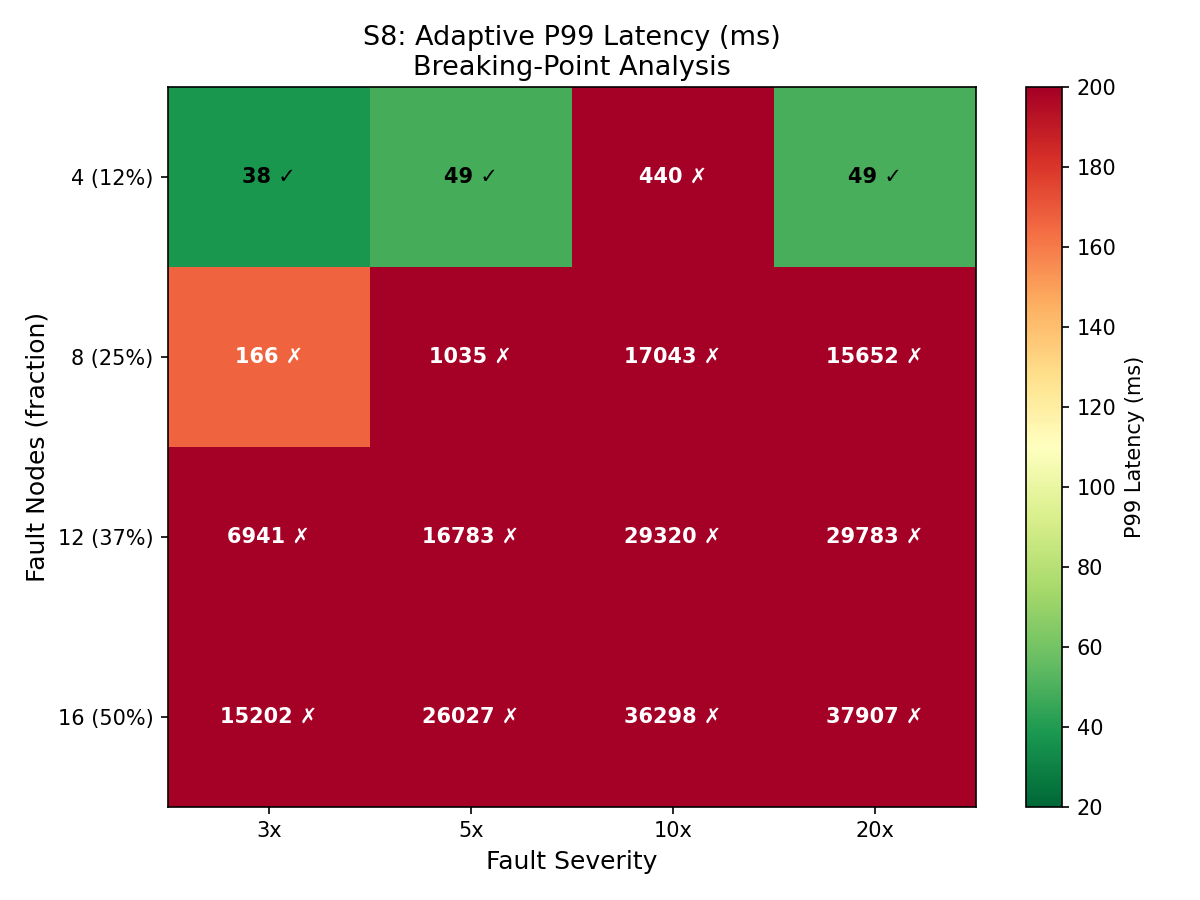
\includegraphics[width=0.85\linewidth]{severity_heatmap.png}
\caption{Severity non-monotonicity heatmap. P99 latency (ms) by fault
  count and slowdown factor at $L = 0.80$, $N = 32$. The
  non-monotonic pattern is clearly visible: for each fault count,
  there exists a critical severity beyond which P99 drops sharply.}
\label{fig:heatmap}
\end{figure}

\subsection{SHED--P2C Complementarity}
\label{sec:complementarity}

The operating envelope and critical severity characterize \emph{what} is
possible. We now analyze \emph{how} P2C interacts with explicit weight
reduction (SHED), showing they are complementary mechanisms---not
redundant.

\paragraph{Two-stage routing under P2C.}
P2C routing makes two sequential decisions:
\begin{enumerate}
\item \emph{Candidate selection:} sample two workers with probability
  proportional to weights $w_i$. The probability of selecting the faulty
  worker as a candidate is approximately $2w_i / \sum_j w_j$.
\item \emph{Queue-depth comparison:} of the two candidates, route to the
  one with the shorter queue.
\end{enumerate}
SHED operates at Stage~1 by reducing $w_i$ for faulty nodes, while P2C's
implicit avoidance operates at Stage~2 through queue-depth comparison.
Stage~2 can only choose between what Stage~1 offers.

\begin{proposition}[SHED--P2C Complementarity]
\label{thm:complementarity}
Under P2C routing with $d = 2$ choices, let $\Delta_{\text{SHED}}(N, s)$
denote the P99 improvement from SHED weight reduction on a single faulty
node with severity $s$ in a cluster of $N$ nodes. Then:
\begin{enumerate}
\item[(a)] \emph{Scale decay:} $\Delta_{\text{SHED}}(N, s) = O(N^{-\alpha})$
  with $\alpha \approx 1.3$ for $s$ in the moderate regime.
\item[(b)] \emph{Severity regimes:} $\Delta_{\text{SHED}}$ is maximized
  at intermediate $s$ (typically $3$--$5\times$), negligible for $s < 1.5$
  and $s > \sstar$.
\item[(c)] \emph{Practical equivalence:} Under P2C, a minimum weight
  $w_{\min} = 0.05$ achieves P99 within $O(w_{\min}/N)$ of full isolation
  ($w = 0$).
\end{enumerate}
\end{proposition}

Intuitively: P2C's queue comparison is already a strong first line of
defense. SHED adds a second filter on top, but because the first line
is already effective, the marginal benefit of the second decays with
cluster size.

\medskip

The proof follows from the two-stage structure. Without SHED (uniform
weights), the probability of the faulty worker appearing as a candidate
per request is $\approx 2/N$. With SHED weight $w_{\min}$, this drops to
$\approx 2w_{\min}/N$---a factor-of-$1/w_{\min}$ reduction in candidacy
rate. However, P2C's Stage~2 already rejects the faulty worker most of the
time via queue comparison. The \emph{net} traffic reaching the faulty
worker scales as $O(1/N)$ without SHED and $O(w_{\min}/N)$ with SHED. As
$N$ grows, the baseline traffic to the faulty worker is already negligible,
so SHED's marginal benefit vanishes.

\paragraph{Capacity-loss boundary.}
The above complementarity has an important exception: when healthy-node
effective load
$L_{\text{healthy}} = L \cdot N / (N - f_{\text{shed}})$ exceeds the
queueing knee ($\approx 0.88$--$0.90$), SHED's weight reduction becomes
counterproductive---the redistributed traffic saturates healthy nodes,
and the resulting queueing delay increase exceeds the original benefit.

\paragraph{Empirical validation.}
Table~\ref{tab:shed_complementarity} validates the complementarity theorem
across cluster sizes, severity levels, and fault counts.

\begin{table}[t]
\centering
\caption{SHED P99 improvement (ms) over no mitigation under P2C.
  SHED reduces weight to $w = \max(0.05, 1-\sigma)$; ISO sets $w = 0$.
  All values are 10-run means.}
\label{tab:shed_complementarity}
\begin{tabular}{@{}lccccl@{}}
\toprule
Config & no\_mit & SHED & ISO & SHED $\Delta$ & Note \\
\midrule
\multicolumn{6}{@{}l}{\emph{Scale sweep ($s = 3\times$, $L = 0.70$)}} \\
$N=8$  & 79.7 & 34.6 & 34.3 & $-45.1$ & Large at small $N$ \\
$N=16$ & 59.3 & 29.8 & 28.2 & $-29.5$ & \\
$N=32$ & 46.6 & 27.8 & 26.9 & $-18.8$ & \\
$N=64$ & 28.5 & 26.8 & 26.4 & $-1.7$  & Negligible at large $N$ \\
\midrule
\multicolumn{6}{@{}l}{\emph{Severity sweep ($N = 16$, $L = 0.70$)}} \\
$s=1.5$ & 29.3 & 28.0 & 28.1 & $-1.3$ & Below detection threshold \\
$s=3$   & 59.3 & 29.8 & 28.2 & $-29.5$ & Peak benefit \\
$s=5$   & 99.7 & 29.7 & 28.2 & $-70.0$ & Near $\sstar$ \\
$s=10$  & 34.6 & 34.6 & 34.6 & $+0.0$ & Above $\sstar$: self-isolated \\
\midrule
\multicolumn{6}{@{}l}{\emph{Without queue-aware routing (weighted random)}} \\
$s=3$, WR & 17757 & 2060 & --- & $-15697$ & SHED critical without P2C \\
\bottomrule
\end{tabular}
\end{table}

The final row demonstrates that SHED is \emph{not} inherently ineffective
---it provides a 15,697\,ms improvement without queue-aware routing. It is
specifically P2C's queue-depth comparison that makes SHED's contribution
marginal. This confirms that the two mechanisms are complementary: P2C
provides the dominant defense, and SHED provides a secondary filter at the
candidate-selection stage.

\medskip

The SHED--ISO gap under P2C is consistently $< 2$\,ms
(Table~\ref{tab:shed_complementarity}), while the gap between no mitigation
and any proactive strategy ranges from 5--70\,ms. This order-of-magnitude
difference implies that the primary engineering challenge is \emph{how
quickly} a faulty node is detected, not \emph{how precisely} its weight is
reduced. A coarse binary detector (``reduce weight or not'') achieves
nearly optimal results under P2C.

\subsection{Implications for Mitigation Design}

The two formulas define three regimes for any $(f, s, L, N)$
configuration:

\begin{enumerate}
\item \textbf{Infeasible} ($f/N > \fmax$): No strategy can maintain the
  SLO. The capacity-theoretic limit is absolute.
\item \textbf{P2C-sufficient} ($f/N \leq \fmax$ and $s > \sstar$):
  P2C's implicit queue-depth avoidance handles the fault automatically.
  Explicit mitigation is unnecessary and may introduce overhead.
\item \textbf{Mitigation-required} ($f/N \leq \fmax$ and $s \leq
  \sstar$): The fault is within capacity limits but P2C cannot
  sufficiently avoid faulty nodes. Proactive detection and traffic
  redirection are needed.
\end{enumerate}

Combined with the complementarity theorem (Section~\ref{sec:complementarity}),
this framework explains when and why explicit mitigation adds value:
\begin{itemize}
\item In Regime~2 ($s > \sstar$), P2C self-isolates faulty nodes. No
  detection or mitigation is needed---but monitoring P999 is critical,
  since high-severity faults remain visible at deeper percentiles.
\item In Regime~3 ($s \leq \sstar$), detection-triggered weight reduction
  or isolation is necessary. Under P2C, the choice between graduated
  weight reduction and full isolation is inconsequential ($< 2$\,ms
  difference). What matters is detection speed.
\item In Regime~1, no strategy helps. The capacity limit is absolute.
\end{itemize}

\section{Reference Implementation}
\label{sec:design}

To evaluate our analytical results, we implement \system{}, a
detection-and-mitigation framework that identifies faulty nodes and
reduces their routing weight. As shown in
Section~\ref{sec:complementarity}, the specific response strategy is
inconsequential under P2C---what matters is detection speed. We
describe \system{} primarily to document the detection mechanism used
in our evaluation.

\subsection{Architecture Overview}

\system{} operates as a control plane alongside the P2C data plane.
Every \emph{decision epoch} $\Delta$ (default 0.5\,s), it executes a
three-stage pipeline: \textbf{Monitor} $\to$ \textbf{Detect} $\to$
\textbf{Act}.

\paragraph{Monitor.}
Collects per-node metrics from the data plane: request departure
intervals, queue depths, and system-wide throughput. Computes
\emph{spare capacity} as the gap between observed throughput and
theoretical maximum, smoothed with an exponential moving average
($\alpha = 0.3$).

\paragraph{Detect.}
Estimates per-node service time from the P10 of inter-departure
intervals---a load-invariant signal derived from M/D/1 queueing theory
(Section~\ref{sec:detection}). Computes severity as:
\begin{equation}
  \sigma_i = \max\left(0,\ 1 - \frac{\tbase}{d_i}\right)
  \label{eq:severity}
\end{equation}
where $d_i$ is the estimated service time of node $i$. A 5$\times$
slowdown yields $\sigma = 0.8$; a 10$\times$ yields $\sigma = 0.9$.

\paragraph{Act.}
Selects a per-node strategy based on severity thresholds and applies
the corresponding traffic adjustment.

\subsection{Detection: Departure Interval Estimation}
\label{sec:detection}

A critical challenge in slow fault detection is distinguishing genuine
degradation from transient queueing effects. At high load ($\rho >
0.85$), all nodes exhibit elevated response times, causing latency-based
detectors to produce false positives.

We exploit a property of M/D/1 queues: when the queue is continuously
busy (which occurs most of the time at high utilization), inter-departure
times equal the actual service time, regardless of queue depth. The P10
percentile of departure intervals filters out idle gaps (when the queue
empties) while capturing the service-time floor.

This signal is \emph{load-invariant}: a node with $\tbase = 10$\,ms
produces $d \approx 10$\,ms whether the system is at 70\% or 95\% load.
A 5$\times$ slowdown produces $d \approx 50$\,ms at any load level.

To prevent transient noise from triggering mitigation, we require
\emph{persistence confirmation}: severity must exceed a minimum
threshold ($\sigma > 0.05$) for two consecutive epochs before a node is
flagged as faulty.

\subsection{Response Strategies}
\label{sec:strategies}

As shown in Section~\ref{sec:complementarity}, under P2C the specific
response strategy has negligible impact on P99 ($< 2$\,ms difference).
\system{} implements three strategies activated by severity thresholds
($\theta_{\text{spec}} < \theta_{\text{shed}} < \theta_{\text{iso}}$):
speculate (send hedged copy to a healthy backup for mildly degraded
nodes), shed (reduce routing weight
$w_i = \max(w_{\min},\, 1 - \sigma_i \cdot \text{spare\_factor})$
for moderately degraded nodes), and isolate (fully exclude severely
degraded nodes, subject to capacity guard $\rhoeff \leq U$).
Isolation is blocked when remaining healthy capacity would exceed $U$.

\subsection{Load-Aware Gating}

The key design principle is that \emph{every mitigation action has a
capacity cost}. Hedging doubles request load; shedding redistributes
load to healthy nodes; isolation removes capacity entirely. At high
system load, these costs can outweigh the benefit, causing the
mitigation trap.

\system{} addresses this through the spare capacity signal, which gates
all three strategies:
\begin{itemize}
\item Hedge budget $\propto$ spare capacity (zero hedges when spare $= 0$).
\item SHED weight reduction $\propto$ spare\_factor (no shedding when
  spare $< 0.08$).
\item ISOLATE blocked when remaining $\rhoeff > U$.
\end{itemize}

This ensures that \system{} gracefully degrades: at low load, it uses
aggressive isolation for fastest recovery; at high load, it uses
conservative shedding to preserve capacity; at overload, it backs off
entirely rather than making things worse.

\section{Evaluation}
\label{sec:evaluation}

We evaluate our analytical results through discrete-event simulation
using SimPy, validated against a JAX-accelerated GPU simulator. Our
goals are to: (1)~validate the operating envelope, severity
non-monotonicity, and SHED--P2C complementarity theorems;
(2)~compare against literature baselines; (3)~characterize robustness
across operating conditions.

\subsection{Experimental Setup}

\paragraph{Cluster.}
$N = 32$ workers, each modeled as an M/D/1 queue with $\tbase =
10$\,ms. Default load factor $L = 0.80$ (total arrival rate
$\Lambda = 2{,}560$ req/s). SLO target: P99 $\leq 50$\,ms.

\paragraph{Baselines.}
We compare eight strategies:
\begin{itemize}
\item \textbf{no\_mitigation}: No response to slow faults (lower bound).
\item \textbf{fixed\_speculation}: Always hedge, never shed or isolate.
\item \textbf{fixed\_shedding}: Always shed load via reduced weights.
\item \textbf{fixed\_isolation}: Aggressively isolate slow nodes
  ($\theta_{\text{iso}} = 0.3$).
\item \textbf{adaptive} (\system{}): Our adaptive multi-strategy framework.
\item \textbf{lit\_hedged}: Unconditional hedged
  requests~\cite{dean2013tail} with delay $= 3 \cdot \tbase$ and
  10\% budget cap.
\item \textbf{lit\_blacklist}: Outlier blacklisting (Cassandra
  style~\cite{lakshman2010cassandra}), $k = 2.0$, cooldown 3 epochs.
\item \textbf{lit\_retry}: Timeout retry with deadline $= 0.7 \times
  \text{SLO}$.
\end{itemize}

\paragraph{Fault scenarios.}
Table~\ref{tab:scenarios} summarizes the 6 primary scenarios (S2--S7),
each exercising a different fault pattern. All use 10 runs with
different random seeds; S4 uses 20 runs due to higher variance from
randomized slowdown factors.

\begin{table}[t]
\centering
\caption{Fault scenarios.}
\label{tab:scenarios}
\small
\begin{tabular}{@{}llccc@{}}
\toprule
ID & Pattern & Faults & Severity & Duration \\
\midrule
S2 & Progressive & 2 & $1{\to}15\times$ & 60\,s \\
S3 & Flash crowd & 2 & $3\times$ + load spikes & 60\,s \\
S4 & Multi-node & 4 & $2{-}5\times$ (random) & 60\,s \\
S5 & Fluctuating & 2 & $5\times$ on/off & 60\,s \\
S6 & Cascade & $1{\to}2{\to}3$ & $5/5/3\times$ & 90\,s \\
S7 & Recovery & 2 & $8\times$ then recover & 100\,s \\
\bottomrule
\end{tabular}
\end{table}

\subsection{Reactive vs.\ Proactive Strategies}
\label{sec:eval-lit}
\label{sec:eval-tiers}

Table~\ref{tab:tiers} presents P99 latency across all scenarios. The
results reveal three distinct performance tiers.

\begin{table}[t]
\centering
\caption{P99 latency (ms) across scenarios at $L = 0.80$. Bold
  indicates best per scenario.}
\label{tab:tiers}
\footnotesize
\begin{tabular}{@{}lcccccc@{}}
\toprule
Baseline & S2 & S3 & S4 & S5 & S6 & S7 \\
\midrule
\system{} & \textbf{30.0} & 39.3 & 43.8 & \textbf{30.3} & \textbf{32.8} & \textbf{29.7} \\
lit\_blacklist & 30.5 & 41.1 & \textbf{37.4} & 30.5 & \textbf{32.8} & 30.5 \\
fixed\_iso & 30.3 & 39.9 & 37.6 & 30.6 & \textbf{32.8} & \textbf{29.7} \\
fixed\_spec & 31.9 & 41.0 & 54.6 & 31.2 & 35.0 & 29.8 \\
fixed\_shed & 33.6 & \textbf{39.2} & 69.3 & 31.1 & 37.0 & 29.9 \\
\midrule
lit\_hedged & 60.8 & 68.2 & 112.9 & 34.6 & 109.9 & 32.3 \\
lit\_retry & 60.8 & 68.1 & 112.7 & 34.5 & 109.5 & 32.3 \\
no\_mitig & 66.7 & 73.5 & 119.5 & 34.9 & 125.3 & 32.3 \\
\bottomrule
\end{tabular}
\end{table}

\paragraph{Tier 1: Proactive strategies (P99 $< 45$\,ms).}
\system{}, lit\_blacklist, and fixed\_isolation all achieve P99 below
45\,ms across every scenario. Their common mechanism---detect faulty
nodes, then stop routing to them---is effective regardless of detection
method (departure intervals, latency outliers, or fixed threshold).

\paragraph{Tier 2: Reactive strategies (P99 $\approx$ no\_mitigation).}
lit\_hedged and lit\_retry provide marginal improvement over
no\_mitigation: SLO violation rates of 0.7--3.4\% vs.\ 0.8--3.7\%
($< 0.3$ percentage points improvement). The root cause: hedging is
designed for random stragglers, not persistent faults. Each request
independently decides whether to hedge, but future requests continue
to be routed to the same faulty nodes.

\paragraph{Tier 3: No mitigation.}
The baseline, with P99 ranging from 32--125\,ms depending on scenario
severity.

Figure~\ref{fig:tiers} visualizes the three-tier separation across all
eight baselines, showing the clear performance gap between proactive
and reactive strategies.

\begin{figure}[t]
\centering

\includegraphics[width=0.85\linewidth]{p99_comparison.png}
\caption{P99 latency comparison across eight baselines (S4 scenario,
  $L = 0.80$). Three performance tiers are clearly visible: proactive
  strategies (P99 $< 45$\,ms), reactive strategies (P99 $\approx$
  no\_mitigation), and the unmitigated baseline.}
\label{fig:tiers}
\end{figure}

\subsection{Minimax Regret at Standard Load}
\label{sec:eval-regret}

Table~\ref{tab:regret} presents the minimax regret analysis across S2--S7.

\begin{table}[t]
\centering
\caption{Minimax regret (ms above scenario-best P99) at $L = 0.80$.}
\label{tab:regret}
\footnotesize
\begin{tabular}{@{}lccl@{}}
\toprule
Strategy & Max regret & Mean regret & Worst scenario \\
\midrule
lit\_blacklist & 0.6 & 0.1 & S7 \\
fixed\_iso & 0.2 & 0.1 & S4 \\
\system{} & 0.2 & 0.1 & S4 \\
fixed\_spec & 9.5 & 2.2 & S4 \\
fixed\_shed & 22.2 & 5.0 & S4 \\
lit\_retry & 76.4 & 36.2 & S6 \\
lit\_hedged & 76.9 & 36.4 & S6 \\
no\_mitig & 92.2 & 42.0 & S6 \\
\bottomrule
\end{tabular}
\end{table}

At standard load ($L = 0.80$), the top three proactive strategies
---lit\_blacklist (0.6\,ms), fixed\_isolation (0.2\,ms), and \system{}
(0.2\,ms)---all achieve near-zero minimax regret. This confirms the
complementarity theorem's key prediction: under P2C, the specific
response strategy matters far less than whether detection occurs at all.

\subsection{SHED--P2C Complementarity Validation}
\label{sec:eval-shed}

We validate the complementarity theorem
(Section~\ref{sec:complementarity}) by comparing P2C-only (no mitigation)
against SHED (weight reduction without isolation) and full isolation
across four dimensions: cluster size, severity, load, and fault count
(S15, 10 runs per configuration).

\paragraph{Scale dependence.}
Figure~\ref{fig:shed_scale} confirms the $O(N^{-\alpha})$ scaling.
SHED's P99 improvement over no mitigation decays from 45.1\,ms at $N=8$
to 1.7\,ms at $N=64$ (1 fault at $3\times$, $L=0.70$). At $N=64$,
P2C alone nearly matches explicit mitigation, consistent with P2C's
candidacy rate of $\approx 2/N \approx 3\%$.

\begin{figure}[t]
\centering
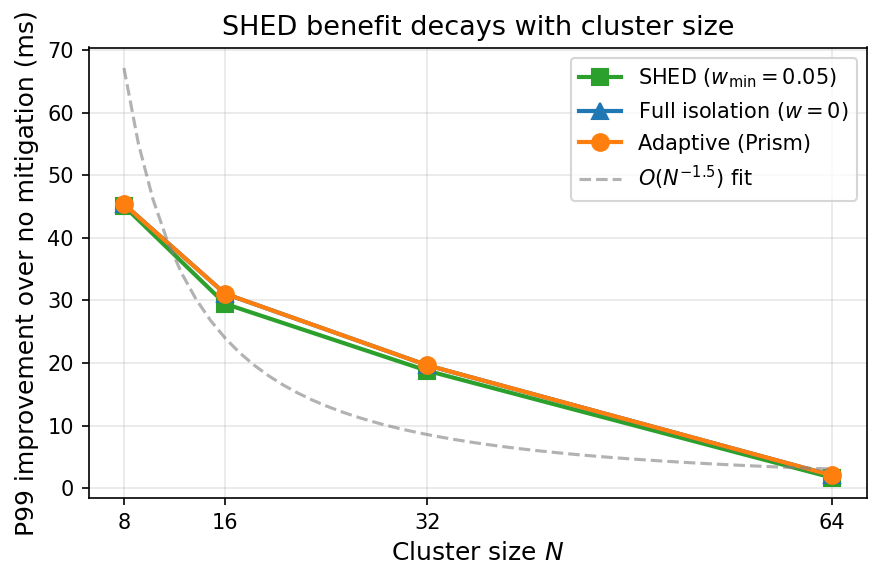
\includegraphics[width=0.85\linewidth]{shed_scale_decay.png}
\caption{SHED benefit decays as $O(N^{-\alpha})$ ($\alpha \approx 1.3$) with cluster size. All
  three proactive strategies (SHED, isolation, adaptive) produce nearly
  identical P99 improvement at every $N$, confirming that strategy
  selection is inconsequential. At $N = 64$, the benefit shrinks to
  $< 2$\,ms.}
\label{fig:shed_scale}
\end{figure}

\paragraph{Self-isolation threshold.}
At $s = 10$ ($N = 16$, $L = 0.70$), all strategies converge to
34.6\,ms: SHED, isolation, and no mitigation produce identical P99. This
confirms that above $\sstar$, P2C's queue-depth signal is sufficient for
complete implicit isolation. The non-monotonicity is stark: P99 rises from
29.3\,ms at $s = 1.5$ to 99.7\,ms at $s = 5$, then drops to 34.6\,ms at
$s = 10$.

\paragraph{SHED $\approx$ ISO under P2C.}
Across all 16 tested configurations, the P99 gap between SHED
($w_{\min} = 0.05$) and full isolation ($w = 0$) is consistently
$< 2$\,ms. In contrast, the gap between no mitigation and either
proactive strategy ranges from 5--70\,ms. This order-of-magnitude
difference confirms that detection is the bottleneck, not strategy
selection.

\paragraph{Control: weighted random routing.}
Under weighted random routing (no queue-depth comparison), SHED provides
massive improvement: 772--15,697\,ms at $s = 1.5$--$5\times$. This
proves SHED's weight reduction is a real mechanism---it is specifically
P2C's queue-depth comparison that makes it marginal. The result
validates that SHED and P2C are complementary rather than SHED being
inherently ineffective.

\begin{figure*}[t]
\centering
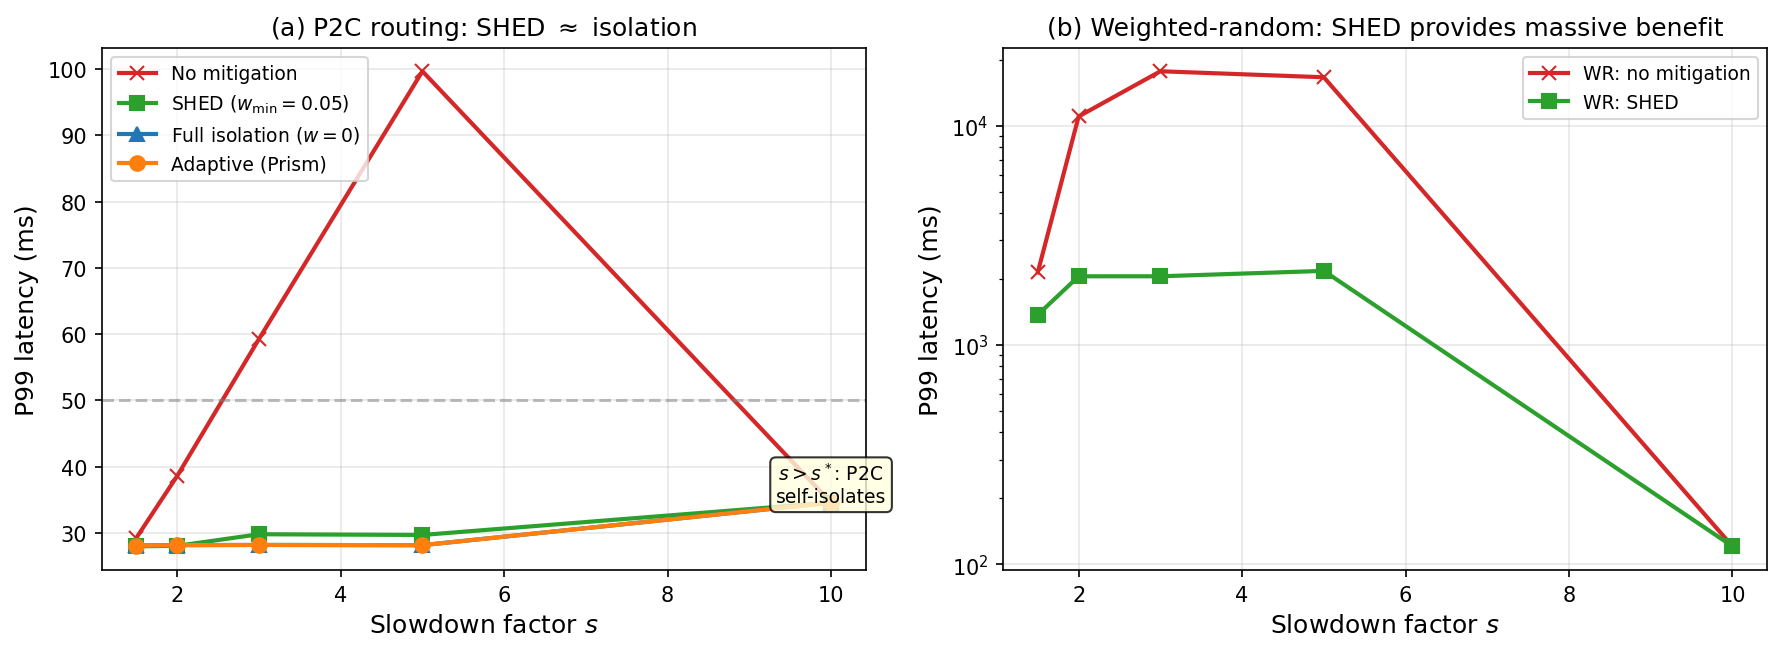
\includegraphics[width=0.95\linewidth]{shed_severity_sweep.png}
\caption{Severity sweep under P2C vs.\ weighted-random routing ($N =
  16$, $f = 1$, $L = 0.70$). (a)~Under P2C, SHED and isolation are
  indistinguishable; the non-monotonicity is clearly visible in the
  no-mitigation curve. (b)~Under weighted-random routing, SHED provides
  order-of-magnitude improvement (note log scale), proving SHED's
  weight reduction is a real mechanism that P2C subsumes.}
\label{fig:shed_severity}
\end{figure*}

\subsection{High-Load Behavior}
\label{sec:eval-highload}

We sweep $L \in \{0.80, 0.85, 0.88, 0.90\}$ across three fault
scenarios (S3-style: 2 nodes/3$\times$; S4-style: 4 nodes/mixed;
S6-style: cascade).

\begin{table}[t]
\centering
\caption{Minimax regret (ms) by load factor across S3/S4/S6 fault
  scenarios.}
\label{tab:highload}
\footnotesize
\begin{tabular}{@{}lcccc@{}}
\toprule
Strategy & $L{=}0.80$ & $L{=}0.85$ & $L{=}0.88$ & $L{=}0.90$ \\
\midrule
\system{} & 7.1 & 90.0 & 26.6 & \textbf{34.8} \\
fixed\_iso & 1.4 & 86.3 & \textbf{18.8} & 34.9 \\
lit\_blacklist & \textbf{0.0} & \textbf{0.2} & 189.7 & 1146.5 \\
no\_mitig & 86.9 & 88.7 & 88.8 & 51.3 \\
\bottomrule
\end{tabular}
\end{table}

\paragraph{Key findings.}
\begin{enumerate}
\item At $L = 0.88$, fixed\_isolation's regret (18.8\,ms) is lower
  than \system{} (26.6\,ms); at $L = 0.90$, the two are nearly tied
  (34.8 vs.\ 34.9\,ms). This further confirms the complementarity
  theorem's prediction: under P2C, strategy choice is inconsequential
  ---graduated response has no systematic advantage over direct
  isolation.

\item lit\_blacklist exhibits \emph{catastrophic failure} at $L \geq 0.88$
  with 4 faults (P99 $= 1{,}407$\,ms, 89\% SLO violation). The root
  cause: blacklisting removes nodes entirely, and its conservative
  cooldown causes oscillation---blacklist $\to$ reintegrate $\to$
  re-blacklist---that amplifies load spikes.

\item At the capacity limit ($L = 0.88$, $f = 4$, $\rhoeff = 1.006$),
  \emph{all} strategies fail, confirming that the operating envelope
  is absolute.

\item In extreme scenarios (e.g., all 8 nodes at $2\times$ fault,
  $L = 0.80$), proactive mitigation \emph{backfires}:
  no\_mitigation (76.3\,ms) outperforms fixed\_isolation (81.7\,ms)
  and adaptive (95.7\,ms). P2C already distributes traffic
  proportionally to capacity; explicit shedding saturates healthy
  nodes. This further confirms the necessity of the operating envelope
  as a prerequisite for mitigation decisions.
\end{enumerate}

\begin{figure}[t]
\centering
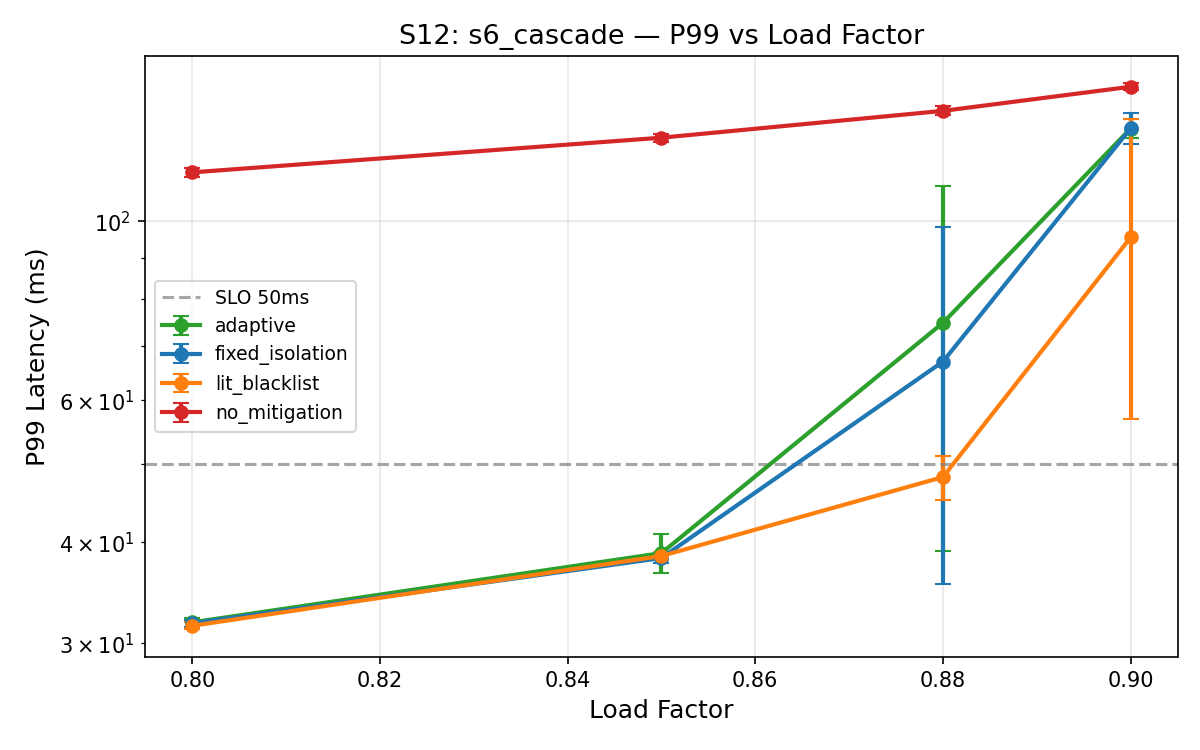
\includegraphics[width=0.85\linewidth]{highload_cascade.png}
\caption{P99 latency vs.\ load factor for the cascade scenario (S6).
  All proactive strategies converge below $L = 0.85$; at $L \geq
  0.88$, the operating envelope is breached and performance degrades
  sharply. lit\_blacklist's oscillation causes it to diverge from other
  proactive strategies at high load.}
\label{fig:highload}
\end{figure}

\subsection{Severity Non-Monotonicity Validation}

Figure~\ref{fig:nonmono} validates the critical severity formula using
S8 data (4 faults, $N = 32$, $L = 0.80$). The predicted $\sstar =
14.1$ for P99 correctly identifies the transition: 10$\times$ (P99 $=
439$\,ms, visible) vs.\ 20$\times$ (P99 $= 49$\,ms, invisible). The
traffic model (Equation~\ref{eq:pfault}) is exact to three significant
figures at $f=8$ and systematically underestimates by 10--14\% at
$f=4$ (see Table~\ref{tab:pfault}).

\begin{table}[t]
\centering
\caption{Severity non-monotonicity at $f = 4$, $N = 32$, $L = 0.80$
  (no mitigation). $\sstar = 14.1$ for P99.}
\label{fig:nonmono}
\footnotesize
\begin{tabular}{@{}cccrl@{}}
\toprule
$s$ & P99 (ms) & P999 (ms) & $\pfault$ & Visibility \\
\midrule
$3\times$ & 95.7 & 118.6 & 5.20\% & Visible ($> 1$\%) \\
$5\times$ & 185.8 & 234.7 & 3.12\% & Visible \\
$10\times$ & 439.0 & 608.3 & 1.56\% & Visible \\
$20\times$ & 49.0 & 17{,}427 & 0.78\% & \textbf{Invisible} ($< 1$\%) \\
\bottomrule
\end{tabular}
\end{table}

The 20$\times$ case is particularly striking: P99 returns to
near-healthy levels (49\,ms), but P999 explodes to 17 seconds because
$s^{*}_{P999} = 142.7$ (well above 20). The fault is a ``silent
killer''---invisible to P99 monitoring but devastating at higher
percentiles.

\begin{figure}[t]
\centering
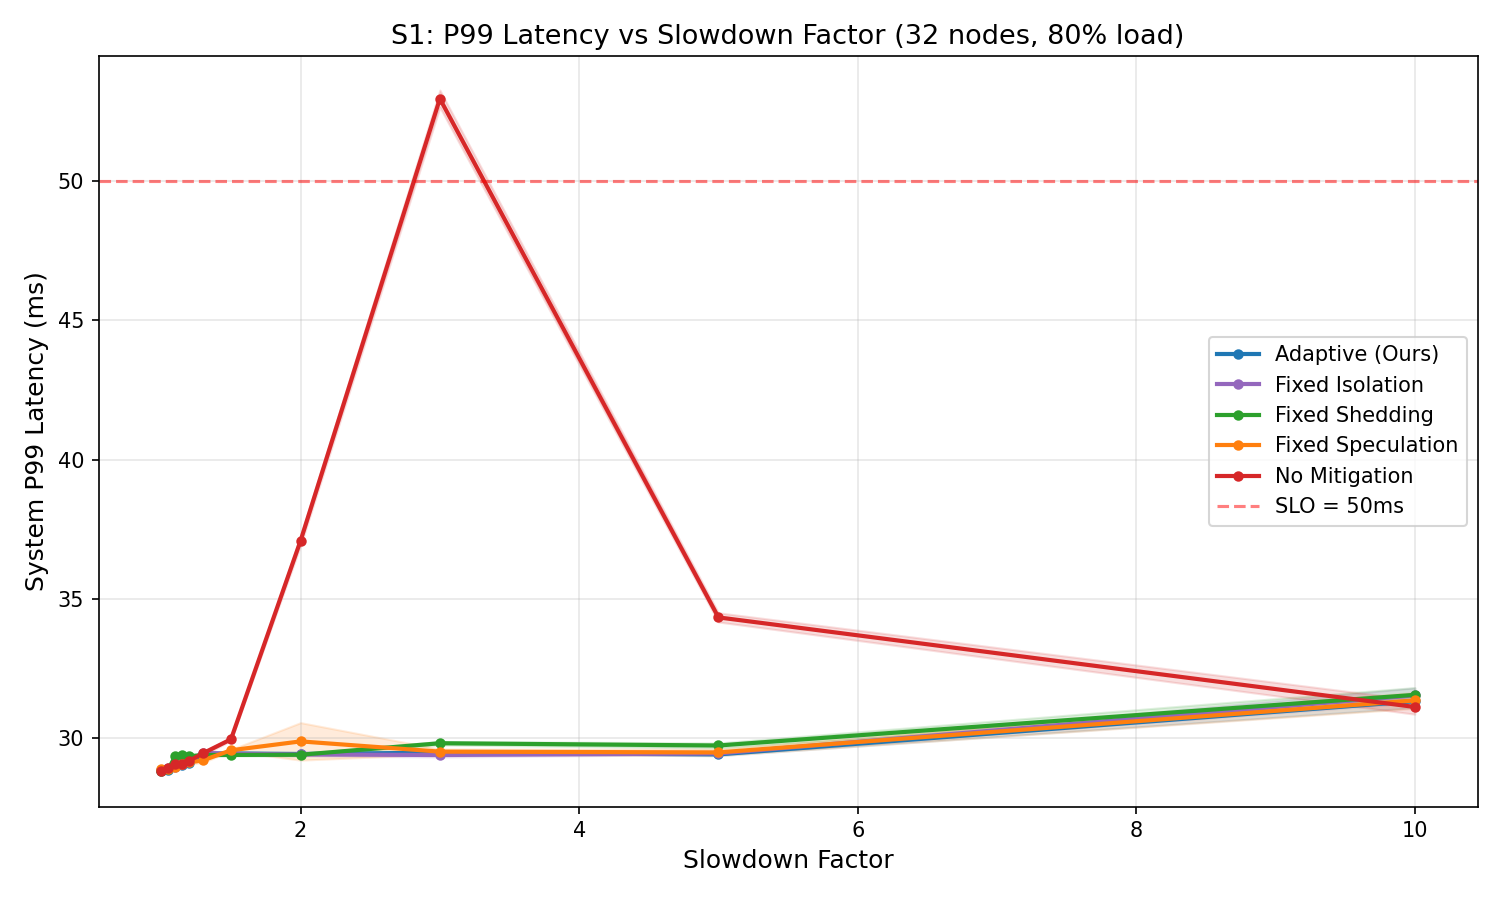
\includegraphics[width=0.85\linewidth]{severity_nonmono_curve.png}
\caption{P99 latency vs.\ slowdown factor ($N = 32$, $f = 2$, $L =
  0.80$). The no-mitigation curve exhibits clear non-monotonicity:
  P99 peaks near $s = 3$ then declines as P2C self-isolates. All
  proactive strategies maintain flat P99 across the severity range.}
\label{fig:nonmono_curve}
\end{figure}

\subsection{Effect of Load Balancing Policy}
\label{sec:eval-lor}

A natural question is whether a more informed load balancer could
replace explicit mitigation. Least-Outstanding-Requests (LOR), which
routes each request to the worker with the shortest queue across
\emph{all} nodes, is theoretically superior to P2C's two-sample
approximation. We compare both policies under three fault scenarios.

\begin{table}[t]
\centering
\caption{P99 latency (ms) under P2C vs.\ LOR load balancing
  ($N = 32$, $L = 0.80$).}
\label{tab:lor}
\footnotesize
\begin{tabular}{@{}llccc@{}}
\toprule
Scenario & Strategy & P2C & LOR & $\Delta$ \\
\midrule
\multirow{3}{*}{S2 (progressive)}
  & no\_mitigation   & 129.7 & 84.3  & $-$45.4 \\
  & fixed\_isolation & 30.8  & 20.7  & $-$10.2 \\
  & adaptive         & 30.8  & 19.9  & $-$11.0 \\
\midrule
\multirow{3}{*}{S4 (multi-node)}
  & no\_mitigation   & 95.9  & 59.2  & $-$36.8 \\
  & fixed\_isolation & 37.8  & 104.4 & $+$66.7 \\
  & adaptive         & 37.7  & 51.2  & $+$13.5 \\
\midrule
\multirow{3}{*}{S6 (cascade)}
  & no\_mitigation   & 126.9 & 83.3  & $-$43.6 \\
  & fixed\_isolation & 32.8  & 20.3  & $-$12.6 \\
  & adaptive         & 32.8  & 19.9  & $-$12.9 \\
\bottomrule
\end{tabular}
\end{table}

Without mitigation, LOR outperforms P2C by 30--45\,ms across all
scenarios: its full-information routing naturally avoids slow nodes.
However, when isolation removes faulty nodes from the pool, the result
reverses in S4 (4 faults): LOR's P99 jumps from 37.8\,ms under P2C to
104.4\,ms. The root cause is \emph{herd behavior}: LOR
deterministically routes all concurrent arrivals to the same
shortest-queue worker, creating synchronized bursts that spike
queueing delay. P2C's randomized two-sample selection provides natural
jitter that prevents this synchronization, making it more robust under
capacity-constrained isolation.

This result explains why P2C---despite being theoretically suboptimal
---is the dominant choice in production systems: its randomness is not
a weakness but a feature that enables safe fault isolation.

\begin{figure}[t]
\centering
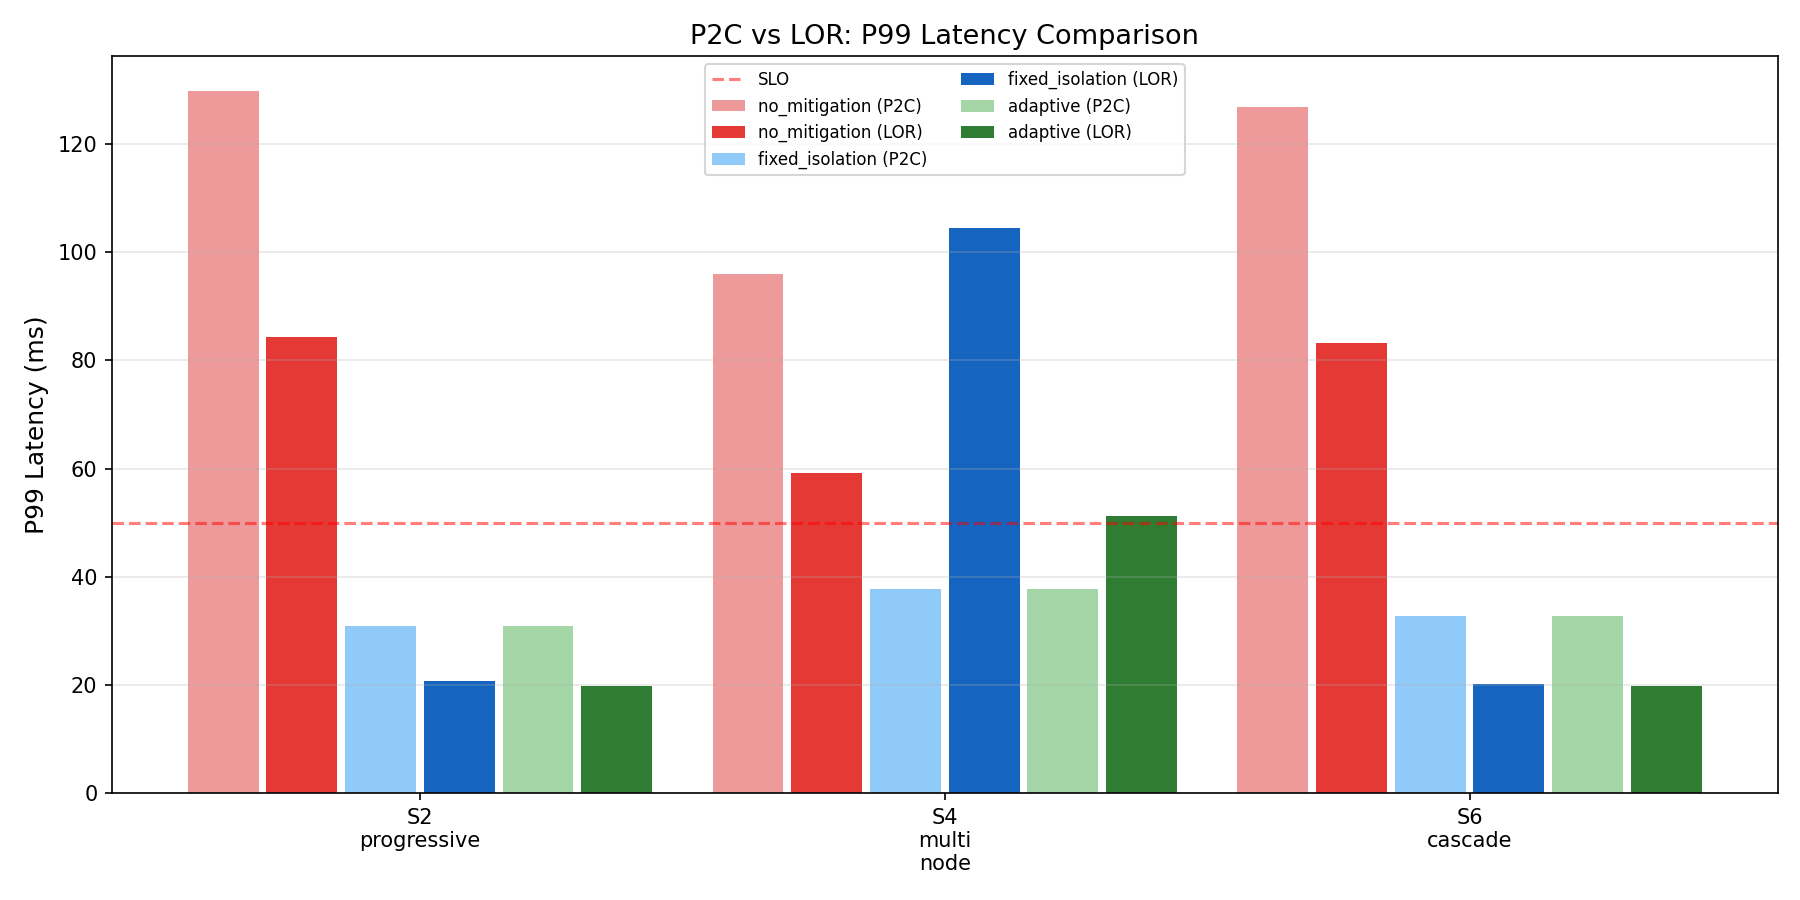
\includegraphics[width=0.85\linewidth]{p2c_vs_lor.png}
\caption{P2C vs.\ LOR across three fault scenarios ($N = 32$, $L =
  0.80$). LOR outperforms P2C without mitigation, but suffers herd
  behavior under isolation in S4 (4 faults): LOR+isolation P99 jumps
  to 104\,ms vs.\ 38\,ms under P2C.}
\label{fig:lor}
\end{figure}

\subsection{Parameter Sensitivity}

We validate that \system{} is not overfitted by perturbing all
thresholds by $\pm 50$\%. Across 13 configurations and 6 scenarios,
all achieve P99 $< 50$\,ms. There is no ``cliff edge'' in parameter
space: performance degrades smoothly, confirming that the framework is
robust to imprecise tuning.

\section{Related Work}
\label{sec:related}

\paragraph{Tail latency mitigation.}
Dean and Barroso~\cite{dean2013tail} established hedged requests and
tied requests as primary tools for tail latency in warehouse-scale
systems. Subsequent work refined these ideas: Vulimiri et
al.~\cite{vulimiri2013low} analyzed redundancy strategies under various
latency distributions; Ananthanarayanan et
al.~\cite{ananthanarayanan2013effective} applied speculation to
stragglers in data analytics. Our work shows that these reactive
mechanisms, designed for random stragglers, are ineffective against
\emph{persistent} slow faults---a distinct failure class requiring
proactive detection.

\paragraph{Gray failure detection.}
Huang et al.~\cite{huang2017gray} characterized gray failures as
differential observability problems and proposed detection via
cross-component correlation. Gunawi et al.~\cite{gunawi2018fail}
cataloged failure modes in cloud systems, finding that performance
degradation accounts for a significant fraction. Our departure-interval
detection builds on this work by providing a load-invariant signal that
distinguishes genuine slowdown from queueing-induced latency increases.

\paragraph{Outlier detection and blacklisting.}
Cassandra's dynamic snitch~\cite{lakshman2010cassandra} uses
exponentially decaying latency scores to route away from slow replicas.
Netflix's adaptive routing~\cite{netflix2020zuul} extends this with
real-time outlier detection. We show that blacklisting is effective at
moderate load but exhibits catastrophic oscillation at high load due to
the capacity cost of node removal.

\paragraph{Load balancing theory.}
Mitzenmacher~\cite{mitzenmacher2001power} proved the exponential
improvement of P2C over random routing for homogeneous servers.
Join-Shortest-Queue (JSQ), also known as Least-Outstanding-Requests,
is optimal for homogeneous systems~\cite{winston1977optimality} but
requires global queue-state information. Our evaluation
(Section~\ref{sec:eval-lor}) shows that JSQ's deterministic routing
creates a synchronization failure mode under fault isolation: when
faulty nodes are removed, all arrivals concentrate on the same
shortest-queue worker, causing herd behavior that P2C's randomized
sampling avoids. We extend the P2C analysis to \emph{heterogeneous}
servers (faulty nodes with different service rates), deriving the
capacity-proportional traffic distribution that underlies the severity
non-monotonicity result.

\paragraph{Capacity planning under failures.}
The $N+k$ redundancy model is standard practice, but the relationship
between load factor, fault fraction, and per-node utilization ceiling
has not been formalized for slow faults specifically. Our operating
envelope formula $\fmax = 1 - L/U$ provides a simple, validated tool
for this purpose.

\paragraph{Adaptive load shedding.}
DAGOR~\cite{zhang2021dagor} and CoDel~\cite{nichols2012codel} address
overload through adaptive shedding, but focus on aggregate system load
rather than per-node fault isolation. Our results show that under
queue-aware routing, the specific response strategy (graduated
shedding vs.\ full isolation) is inconsequential ($< 2$\,ms P99
difference); detection speed is the key bottleneck. This contrasts
with the above works' emphasis on response strategy design.

\section{Conclusion}
\label{sec:conclusion}

We presented a capacity-theoretic analysis of slow fault mitigation
under Power-of-Two-Choices load balancing, establishing three results.
The \emph{operating envelope} ($\fmax = 1 - L/U$) determines when
mitigation is feasible. The \emph{critical severity} ($\sstar =
fq/((1-q)(N-f))$) identifies the slowdown regime where P2C's implicit
avoidance suffices versus where explicit detection is needed. The
\emph{SHED--P2C complementarity} (Proposition~\ref{thm:complementarity}) shows that under queue-aware
routing, detection speed dominates strategy selection: graduated weight
reduction and full isolation achieve nearly identical P99, and the
benefit of any explicit mitigation decays as $O(N^{-1.3})$ with cluster
size.

Our evaluation across 15 fault scenarios yields two actionable findings:
(1)~reactive mechanisms (hedged requests, timeout retry) are ineffective
against persistent slow faults; (2)~proactive detection with traffic
exclusion is both necessary and sufficient, with the specific exclusion
mechanism being inconsequential under P2C.

The severity non-monotonicity result has a practical implication:
monitoring dashboards that track only P99 latency will miss faults with
$s > \sstar$, which appear normal at P99 but are catastrophic at P999.
Systems should monitor multiple percentiles to detect these ``silent
killers.''

\paragraph{Limitations.}
Our model assumes a single-tier architecture with homogeneous workers
and no request affinity. Multi-tier systems with fan-out amplify slow
fault impact~\cite{dean2013tail}, and we expect the operating envelope
to tighten. The utilization ceiling $U$ is derived from mean latency
(Corollary~\ref{cor:U}); for the M/D/1 model used throughout, the
formula is conservative. For high-variance service times ($\Cs^2 \geq 1$),
the mean-based $U$ is optimistic (Remark~\ref{rem:mean-p99}). The
SHED--P2C complementarity result applies specifically to P2C; under
non-queue-aware routing (weighted random), SHED provides massive benefit
(Table~\ref{tab:shed_complementarity}), suggesting the result does not
generalize to all routing policies.

\paragraph{Future work.}
Two directions are natural extensions. First, \emph{retry amplification}:
retries under slow faults increase effective load by
$L_{\text{eff}} = L \cdot (1 + r \cdot p_{\text{timeout}})$, potentially
shrinking the operating envelope. Formalizing how retries interact with
the capacity limit is important for systems with retry policies. Second,
extending the analysis to \emph{fan-out architectures}, where a single
slow node affects $O(N)$ requests through scatter-gather, likely reduces
tolerance to $\fmax \approx (1-L/U)/\text{fan-out}$.


\bibliographystyle{plain}
\bibliography{references}

\end{document}
